%%document preambel

\documentclass{scrartcl}
\usepackage[ansinew]{inputenc}
\usepackage[T1]{fontenc}
\usepackage{graphicx}
%\usepackage{beramono}% monospaced font with bold variant

%\usepackage{listings}
%\lstdefinelanguage{VHDL}{
%  morekeywords={
%    library,use,all,entity,is,port,in,out,end,architecture,of,
%    begin,and
%  },
%  morecomment=[l]--
%}
%
%\usepackage{xcolor}
%\colorlet{keyword}{blue!100!black!80}
%\colorlet{comment}{green!90!black!90}
%\lstdefinestyle{vhdl}{
%  language     = VHDL,
%  basicstyle   = \ttfamily,
%  keywordstyle = \color{keyword}\bfseries,
%  commentstyle = \color{comment}
%}


\begin{document}

\title{Partial reconfiguration and fault simulation on Altera Cyclone FPGA}
\subtitle{Students project at the chair of computer architecture university freiburg}
\author{Markus Wei�}
\maketitle
\tableofcontents
\newpage

\section{Software prerequisites}
The software used in both projects were Quartus II Version 14.1/15.0 and QSYS on Windows 7/8.1.\\Quartus II is a design software for FPGAs (field programmable gate array) of Altera. With Quartus II VHDL- files were generated. The Quartus II software can be configured to reach different design goals, e.g. time complexity, speed, optimization of compilation time or energy consumption.\\ QSYS is described as a tool for system integration, to safe time by generating automatic connection-logic for different components. The developed VHDL code from Quartus II software can be imported to QSYS and is processed there to connect different components on the dev kit board. QSYS has to initiate, configure and connect the hps (hard processor system) to the fpga if they need to communicate.\\ In addition to the development software some driver have to be installed on the running operating system. To program the FPGA via the USB cable a special driver, Altera USB Blaster driver, needs to be installed. The installation of the Altera USB Blaster driver was not so intuitive as expected, cf. 3.5 problems.\\
The following software is used:
\begin{itemize}
	\item Windows 7/8.1 	
	\item Quartus II (Version 14.1/15.0)
	\item QSYS
	\item Altera USB Blaster driver (insert version or revision)
	\item portable os for the dev kit (partial reconfiguration)
	\item usb-to-serial converter driver (fault simulation)
\end{itemize}
\newpage
\section{Partial reconfiguration}
\subsection{Prerequisites}
The hardware used in this project was a development kit board from altera, namely "Terasic DE1-SoC Development Kit". This board consists of the following core components: an FPGA, named Altera Cyclone V (5SCEMA5F31C6N), a dual-core Cortex-A9 (HPS), 1GB DDR3 and 64MB SDRAM memory and different interfaces like USB,JTAG and i2c.\\ The communication interfaces are a on board USB-Blaster II, USB 2.0 ports, UART interface, Ethernet port and extended module for GPIO (general purpose input/output) pins.\\
The FPGA is the mainly used component of the development kit board and therefore here are some useful facts about it (Cyclone V):\\
\begin{itemize}
	\item 85000 logic cells on the board
	\item 4450 kb embedded memory
	\item access to an external 64 MB static random access memory (SRAM)
	\item low energy consumption
\end{itemize}
The Cyclone V is configured through the USB Blaster interface, where a bit stream is loaded to the memory of the board. This bit stream is lost once the energy is off.
Alternatively an in-system NOR flash memory can be loaded with this bit stream, which safes it although the power is taken off.\\ Another way to configure the FPGA is to use the hard processor system (hps). This is done either while the boot process, with "U-Boot" or the "preloader", or after the operating system is fully booted.\\ While booting the preloader initiates the clock, is responsible for multiplexing pins, configures the main memory and loads the U-Boot.  The configuration of the main memory of the hard processor system and the AXI Bridges is crucial, because these have to grant the FPGA access.\\ The universal boot loader initiates and tests hardware components. Also it downloads and executes application software. This boot-loader is required to initiate the boot process of the UNIX-kernel. \\ To get access from the FPGA to the main memory of the hps the Avalon-Memory-Mapped-Interface has to be configured. It enables efficient read- and write operations, interrupts, clocks, resets and control progresses. This Avalon-MM-Interface enables address based read- and write procedures in a master/slave connection.\\
To start a C++ program on the board an operation system for the hps is needed. The used operation system was a small sized portable linux system (KERNEL VERSION???) which was loaded to an sd card. 
\subsection{The idea and the benefit}
The concept of partial reconfiguration is highly desirable for some special purposes. 
With this feature it would be easier to change partially designs or improve the functionality of an FPGA without interrupting its work progress. 
Special applications may need to change some logic on an FPGA while another part of it is not allowed to stop. 
For example it is crucial to establish a reliable flow of data without interrupting it while another part of the FPGA can still change its logic.
Therefore this concept is desirable in the field of communication systems. 
A benefit of this idea is that the number of devices can be scaled down, therefore the power consumption and the cost can be reduced. 
The tasks two or more FPGAs has handled before can now be handled by one FPGA due to the fact that only a small part of the FPGA is changed while the other part is still running.\\
The partial reconfiguration concept in this project is initialized by an internal host. The internal host starts the process of reconfiguration. For this the processor on the development kit (hps) programs the desired locig cells of the FPGA while the other part of the logic cells remains.
% This initiation is done by an internal host which runs a C/C++ program. This C/C++ program is stored in the RAM (read access memory) of the development kit board.\\
Partial reconfiguration in combination with the fault simulation explained later, give a high speed and efficient way to detect faults in hardware.

\subsection{Design flow and implementation}
The focus of the partial reconfiguration is rather on logic blocks than DSP, memories, PLL, transceivers and I/O blocks. Functions in the periphery like GPIO or I/O registers can not be partially reconfigured.\\ 
For the partial reconfiguration of logic blocks two different regions in the top level design are needed.
One static region, which continues its process and one region, which can be dynamically configured.
To get an optical feedback of this configuration process, two led pattern are generated. One pattern, in the static region, highlights the leds to check if the FPGA is still running while another led pattern is loaded to the dynamic region which let us check if the other part of the FPGA is reconfigured.\\
To avoid errors in the in- and output of the gates, a wrapper region is needed. This region is generated to ensure that all personas, e.g. led pattern, have the same connection to the static region. This can be done by creating dummy ports.\\
For partial reconfiguration all non-global inputs of the pr regions must be freezed. Freezing means in this context to drive a '1' to the inputs, which ensures there is no contention between current values and those after partial reconfiguration. Therefore a freeze region is essential.\\In this project a partial reconfiguration with an internal host is realised, which initializes the reconfiguration with a c/c++ program. 
For this purpose the processor has to communicate with the FPGA and with the memory. The communication between the hard processor system and  the FPGA, the main memory and in- and output interfaces is a very important point.\\
A short description of the projects design flow is listed here:
\begin{enumerate}
	\item planning the system for partial reconfiguration
	\item identify which blocks to reconfigure 
	%$\rightarrow$ led pattern for the led on DE1-SoC board
	\item code the design in Quartus II
	\begin{itemize}
		\item develop the personas
		\item generate static and pr region
		\item generate freeze and wrapper region
	\end{itemize}
	\item connect components with QSYS
	\begin{itemize}
		\item assign partitions to logiclock regions
	\end{itemize}
	\item create necessary files to program FPGA with Quartus II
	\item program FPGA via USB Blaster 
\end{enumerate}
Quartus II creates the logic in VHDL, while QSYS connects different system components which communicate and access each other. This informations are required to generate the "preloader" which coordinates the boot process. 
%The next step of booting is the "universal boot loader" which configures the fpga and load the "linux-kernel". The Avalon-MM-Interface is required to grant the fpga access to the main memory of the HPS.\\

%Two different led pattern, a wrapper and a freeze region were designed. The design partition were associated with the logiclock regions of the fpga
%	\item connect I/O signals with pins (QSYS)


%There are different options for the communication between HPS and FPGA, which are mentioned here: 
%\begin{enumerate}
%	\item Advanced extensible interface bus bridges (AXI)
%	\begin{enumerate}
%		\item Lightweight HPS-to-FPGA bridge
%		\item HPS-to-FPGA bridge
%		\item FPGA-to-HPS bridge
%	\end{enumerate}
%	\item FPGA-to-SDRAM
%\end{enumerate}

%\\ Project design flow, hierarchy etc, code citation.
%Which design blocks are necessary to program the fpga for partial reconfiguration. Wrapper, logic, etc. ...comment on created code.

\subsection{Problems}
Two crucial problems occurred during the work on partial reconfiguration.
\begin{enumerate}
	\item  No permission to use partial reconfiguration feature in Quartus Software
	\begin{itemize}
		\item a new license was inquired
	\end{itemize}
	\item the FPGA Cyclone V does not support the feature of partial reconfiguration
	\begin{itemize}
		\item could not be solved because a new FPGA was not affordable
	\end{itemize} 
\end{enumerate}
After working 8-10 weeks on this topic the project has to be stopped due to the fact that partial reconfiguration is not supported by FPGA. At this time the status quo was:
\begin{itemize}
  	\item literature survey
  	\item soft- and hardware prerequisites
  	\item project design flow
  	\item creating different revisions for partial reconfiguration in Quartus II
  	\item VHDL design
	\begin{itemize}
		\item top level
		\item wrapper
		\item freeze region
		\item static region + personas
		\item partial reconfiguration region + personas
	\end{itemize}
	\item assignments with QSYS
	\begin{itemize}
		\item logic lock region assignments
		\item pin assignments
	\end{itemize}
  \item file creation for programming the fpga (.pmsf, .msf, .sof, .rbf)
\end{itemize}
There is a slightly different approach to program the FPGA with partial reconfiguration. There a couple of files are needed and loaded to the FPGA. Therefore the files have to be created using the Quartus II software.
\subsection{Discussion/Conclusion}
Researching this topic is totally worth it. Partial reconfiguration can be used in time critical systems, like communication systems, where an abrupt stop of a data flow is critical. It is a nice way to improve configuration speed, because another part can still run. The field of partial reconfiguration is still a new topic in research and development and yet it is not integrated in industrial products. The main disadvantages are the cost of a special FPGA and special software instead of using an cheaper fully developed ASIC, and a lot more time must be spent on validation.
\newpage
\section{Fault simulation}
\subsection{Prerequisites}
The hardware used in this part of the project was a former dev kit from altera with a fpga Cyclone IV.\\
In addition to the software mentioned in section 1, there is some special software required for this part of the project:
%In addition to the mentioned software in the beginning some special software is required:
\begin{itemize}
	\item C++ compiler e.g. MinGW to compile C++ files to *.exe files
	\item USB-to-Serial driver to get a connection between dev kit to pc via serial interface RS232
\end{itemize}
Also a couple of files from a former project of two students were provided. This part of the project is based on the former work and extends it.
\subsection{Idea and benefit}
The idea of fault simulation is to detect stuck-at faults in an efficient way in hardware. This increase the fault detection speed and therefore much more faults can be detected in shorter time periods. The concept is to compare a test pattern with a original circuit under test with a changed circuit under test. Therefore a special test pattern is loaded to the ram of the FPGA via USB Blaster. The circuit under test is realized by two different circuits. One circuit without fault pattern and one with changed logical cells. The output of both circuits is lead to a logical XOR gate which identifies if an error is detected or not. If the outputs of both circuits distinguishes the XOR gate give a logical one, hence a fault. Otherwise no fault is detected. This output is saved into a FIFO (first in first out) memory and then transmitted to the pc for documentation. For this communication link the usb to serial connection is needed.\\
%Efficient fault simulation in hardware FPGA. modification of the circuit with special changes to the look up tables. evaluation and pc communication with serial interface rs232.\\
%To detect faults some lcells are modified. 
% \textbf{lcell}
% \begin{itemize}
%	\item smallest logic cell
%	\item maximal four inputs
%	\item gatter are ordered in a logic cell
%	\item every lcell have a look-up table, which defines the output
%	\item the function of a particular  lcell can be changed by hand
%\end{itemize}
The idea of the Maximum fanout free cones (MFFC), adopted from a former project,   is to assign as many as possible gates to one logic cell. This would reduce the size used for this circuits. The creation of maximum fanout free cones is an algorithm to minimize the number of gates in one logic cell. This algorithm is implemented by a the former work of two students.
% The look-up table (LUT) can be calculated for every locig cell in Quartus. The evaluation is done over the rs232 interface and a personal computer. 
The goal is a very fast and efficient way to detect faults.


\subsection{Preparation and process to execute the fault simulation}
After setting up the software prerequisites you can try to run the project. This list shows the process to execute the fault simulation on the FPGA: 
\begin{enumerate}
	\item compile quartus project
	\begin{itemize}
		\item open 'FaultInjectionTester.qar' with Quartus II
		\item compile this project
		\item close Quartus II
	\end{itemize}
	\item create IRA.exe in root folder (make.batch file)
	\begin{itemize}
	\item open command window and change directory to FaultConfiguration
	\item execute: \textit{g++ IRA.cpp CGate.cpp CGate.h CComponent.h -o ..IRA.exe}	
	\end{itemize}
	\item create FaultInjectionTester.exe in root folder (make.batch file)
	\begin{itemize}
	\item open command window and change directory to FPGACommunication
	\item execute: \textit{g++ FaultInjectionTester.cpp PcFPGACommunication.cpp PcFPGACommunication.h -o .."FaultInjectionTester.exe"}
	\end{itemize}
	\item Connect board and pc via USB Blaster
	\item connect board and pc via RS232
	\item execute IRA.exe [path to quartus], e.g. IRA.exe "C://Program Files//Altera"
\end{enumerate}
If it all worked well, the pc programs and tests the fpga. The communication link is via the RS232 interface, for which the usb to serial driver is necessary.\\
Otherwise following common errors can occur while executing:
\begin{itemize}
	\item "Can not find quartus\textunderscore cdb"
	\item "Inconsistent set or reset compile started variable"
\end{itemize}
For a solution see \ref{problemandtroubleshoot}.

%explain the complete process:
%\begin{enumerate}
%	\item TCL script
%	\item batch
%	\item quartus project
%	\item c++ files
%	\item exe files
%	\item vhdl files
%\end{enumerate}

\subsection{Implementation and improvement}
To enhance the existing project a batch file was created which automates the process of generating the executable files.
This makes it easier in a more convenient way to set up the project and make it ready for execution. 
Another step in the working progress was to change absolute paths to relative paths, so it can be used by everyone without checking the cpp program files.
Then an error was detected in the design flow which leads to false results. 
This error cost very much time to find and it must be figured on finding other errors in the design flow. 
This shows that the previous work was not final and that there could be more errors.
%It takes a lot of time to debug the former code. 
A bunch of weeks was invested on debugging and struggling with several software installation problems to run the projects files on the FPGA.\\
The improvements and changes which were made in an overview:
\begin{itemize}
	\item changed absolute paths to relative paths
	\item code debugging
	\item clear faults in design flow 
	\item create a batch file to automate process
\end{itemize}


\subsection{Problems and troubleshooting} \label{problemandtroubleshoot}
Debugging and troubleshooting several errors became the main part of this project. Here are the problems mentioned which occurred during the project.
\begin{enumerate}
	\item \label{p1} driver installation of USB Blaster II
	\item \label{p2} driver installation of FTDI Chip for USB-Serial converter
	\item \label{p3} error in the design flow
	\item \label{p4} errors while execution
	\begin{enumerate}
		\item \label{p4.1}"inconsistant set or reset of compile started variable"
		\item \label{p4.2} "quartus\textunderscore pgm could not be found" - [insert SCREENSHOT]
	\end{enumerate}
\end{enumerate}

%\begin{enumerate}
%	\item driver installation of USB Blaster II
%\end{enumerate}
\ref{p1} Also it seems to be intuitive to install a USB driver, it was quite difficult to install in Windows 8.1 x64 pro. Although it is an official driver from Altera Windows 8.1 x64 pro does not support this driver because it has no driver signature. First of all the following problem was encountered : 
\begin{figure}[!ht]
	\centering
  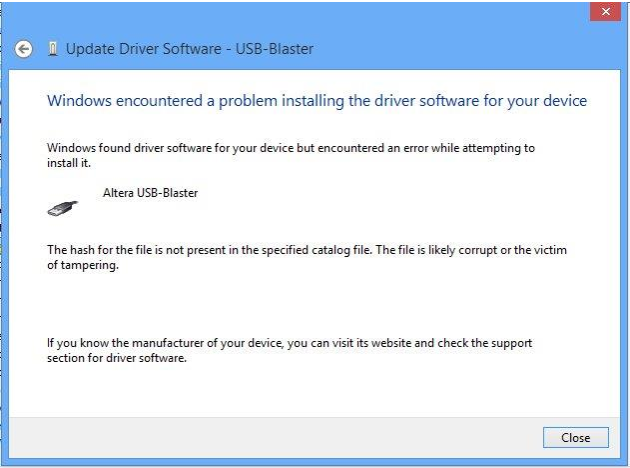
\includegraphics[width=0.8\textwidth, angle=0]{USB_blaster_driver_problem.png}
	\caption{failed installation of usb blaster driver}
	\label{usbblasterproblem}
\end{figure}
Neither the installation of the driver on the system cd nor the newest driver from alteras homepage could solve this problem. The attempt of windows to install this driver ended in the error in fig. \ref{usbblaster2}.
\begin{figure}[!ht]
	\centering
  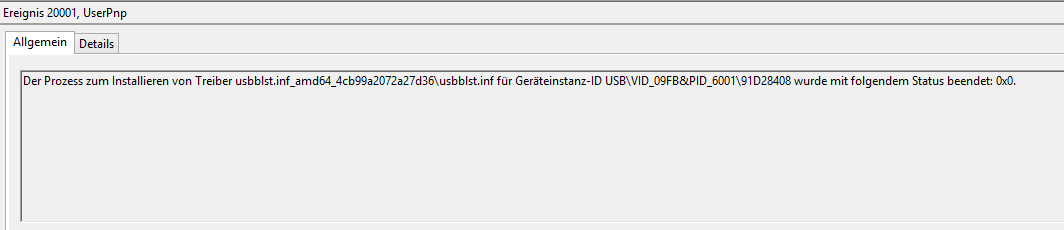
\includegraphics[width=1\textwidth, angle=0]{USB_blaster_problem2.png}
	\caption{AlteraUSBBlaster install not successfull}
	\label{usbblaster2}	
\end{figure}

After searching for a while in alteras forum and the internet to this problem, the solution was found on: \textbf{\textit{http://altera-guide.blogspot.de/2012/11/many-collage-students-find-ourselves.htmlcomment-form}}\\
Figure \ref{installguide} shows the screenshot from the blog entry to solve this problem.\\

After successfully installing the driver, another problem may occur while starting the driver, see fig.\ref{usbblaster1}:
\begin{figure}[!ht]
	\centering
  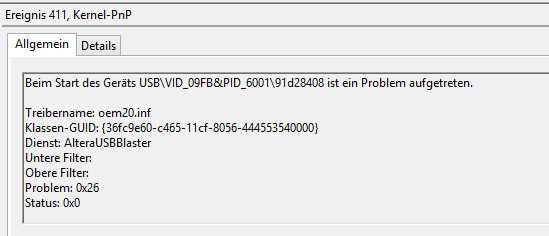
\includegraphics[width=1\textwidth, angle=0]{USB_blaster_problem.png}
	\caption{AlteraUSBBlaster problem}
	\label{usbblaster1}	
\end{figure}
It seems to be correlated to the driver installed but that is not exactly validated .

\ref{p2} If the USB Blaster driver was successfully installed, there came another problem concerning the usb to serial conversion for the communication link between pc and dev kit. The driver could not be installed and hence it could not be started see Fig. \ref{usb_serial_problem} and \ref{ftdi_problem1}

\begin{figure}[!ht]
	\centering
  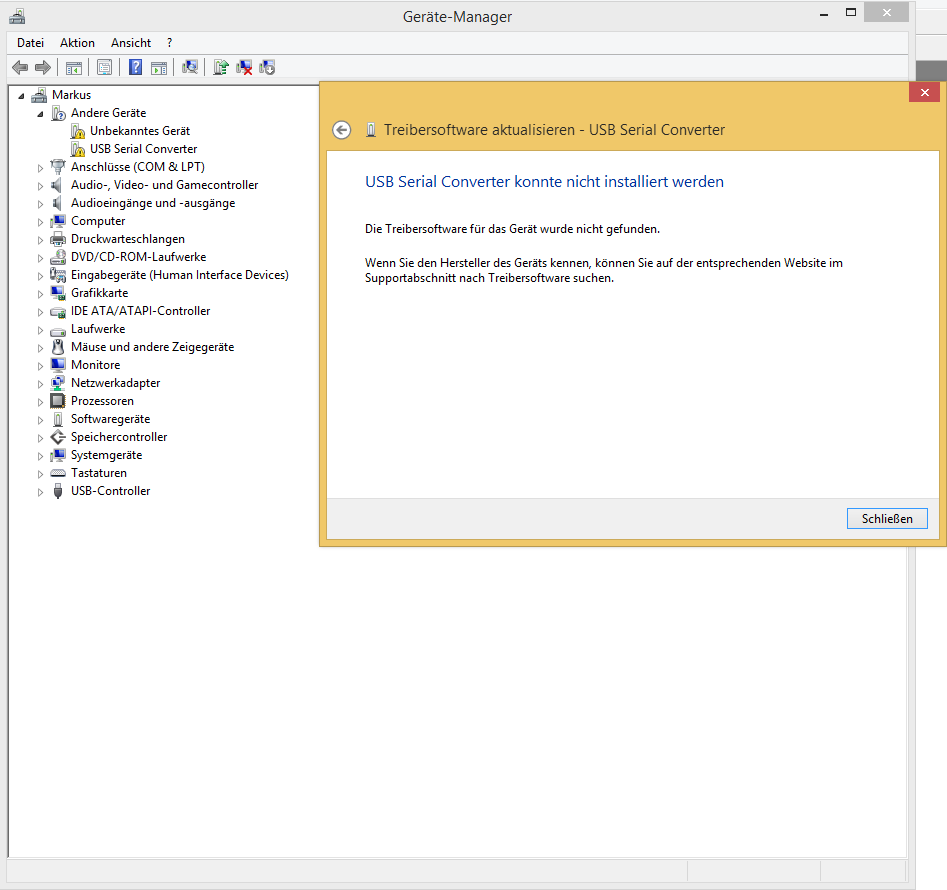
\includegraphics[width=1\textwidth, angle=0]{USB_serial_driver.png}
	\caption{USB Serial Converterter could not be installed}
	\label{usb_serial_problem}	
\end{figure}

\begin{figure}[!ht]
	\centering
  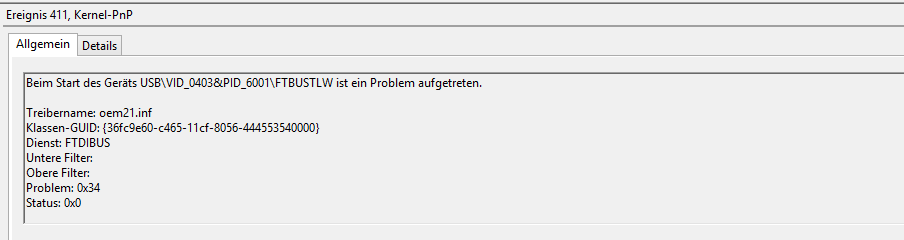
\includegraphics[width=1\textwidth, angle=0]{FTDI_USB_SERIAL_CONVERTER_problem.png}
	\caption{FTDI chip problem}
	\label{ftdi_problem1}
\end{figure}
If you try to install the driver with the standard windows application you run into this problem, see Fig. \ref{ftdi_problem2}

\begin{figure}[!ht]
	\centering
  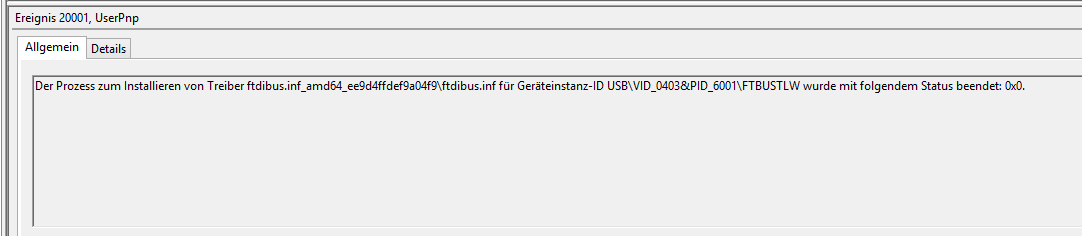
\includegraphics[width=1\textwidth, angle=0]{FTDI_USB_SERIAL_CONVERTER_problem2.png}
	\caption{Driver install not successful}
	\label{ftdi_problem2}	
\end{figure}
 In the end the driver for the FTDI Chip was searched in the internet and installed. 
\ref{p3}
There was an error in the design flow of the former work. It was realised that there was no compilation after changing LUTs of circuit under test.\\
If all the troubleshooting about the installation of different drivers were made another error was detected while executing the project.\\
\ref{p4.1} The execution error occuring while execution was:
\begin{figure}[!ht]
	\centering
  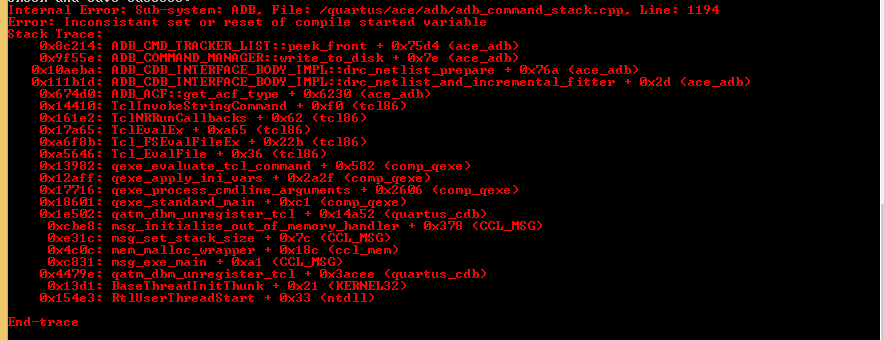
\includegraphics[width=1\textwidth, angle=0]{inconsistent_set.png}
	\caption{inconsistent set}
	\label{inconsistentset}	
\end{figure}
To solve this, you have to follow this:
\begin{enumerate}
	 		\item clear out the "db" and "incremental\textunderscore db" folder in "FaultInjectionTester\textunderscore restored" folder
		\item recompile Quartus project
		\item execute IRA.exe once more
\end{enumerate}

\ref{p4.2}
If an error message appears which states that a quartus\textunderscore pgm or cdb or whatever could not be found, you have to check the path of your quartus installation.

\newpage
\subsection{Discussion and future work}
Debugging and troubleshooting become the main part of the project. A lot of problems occurred during this work. These problems prevented a learning process in vhdl, which was the intend to do a project at the chair of computer architecture. The second part of the project was a project in the programming language of C++ and hence none of hardware programming.\\
The workstation for this project was a desktop pc and not a  laptop, which makes it difficult to share the problems like driver issues with the other guys. \\
The best way to enhance this project were to set up the whole project on a virtual machine. So there could not occur any software issues and the project can be run independently of any operating system. There should be only one supported software version of Quartus II and QSYS and also a version control feature for the project. The version control is needed if a group should work with this project.
This setup would have taken too much time in the workload of this project but it would be a nice part for future work.
\\

% path to installed software. troubleshooting for installation of usb blaster driver. debugging former code fractions. error in design flow (compilation missing after changing luts). creating batch file to automate it. relative paths to automate. further improvements: design for a virtual machine, version control. 
%All in all i can say to work on a proper design is very difficult.
%The communication link between RS232 and Board work properly, but without the information on the Version of used software (quartus, qsys, operating system etc.) it is too difficult.
%Also the installation path should not be absolute.
%%There were an error that the project was not compiled after changing the LUTs. 
\begin{figure}[!ht]
	\centering
  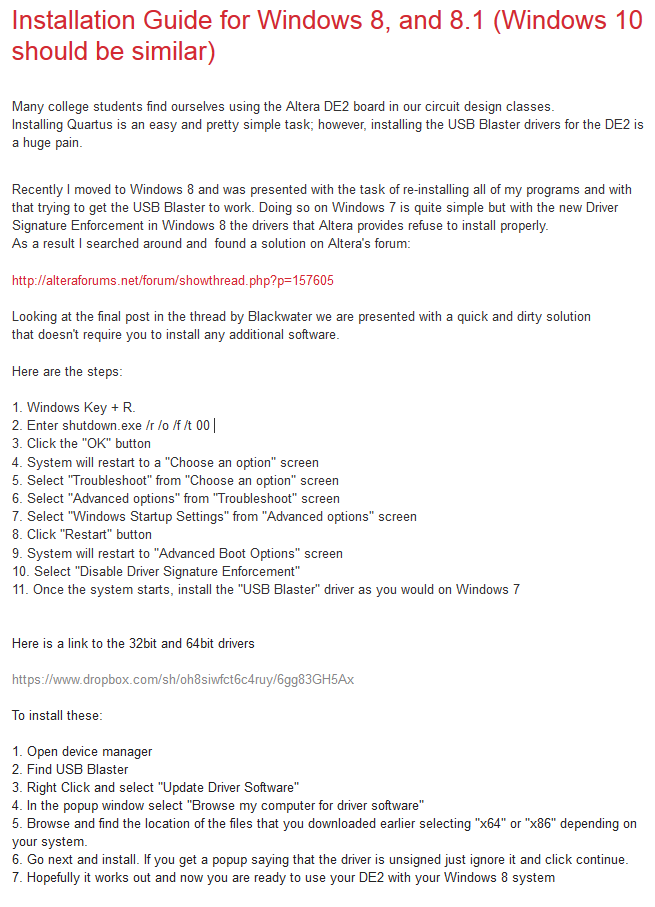
\includegraphics[width=1\textwidth, angle=0]{installationGuide.png}
	\caption{steps to install the usb driver}
	\label{installguide}
\end{figure}
\end{document}
